\documentclass[conference]{IEEEtran}

\usepackage{cite}
\usepackage{amsmath,amssymb,amsfonts}
\usepackage{algorithmic}
\usepackage{graphicx}
\usepackage{subfigure}
\usepackage{textcomp}
\usepackage{xcolor}
\usepackage{tabularx, booktabs}

\newcolumntype{L}{>{\centering\arraybackslash}m{2cm}}

\def\BibTeX{{\rm B\kern-.05em{\sc i\kern-.025em b}\kern-.08em
    T\kern-.1667em\lower.7ex\hbox{E}\kern-.125emX}}
\begin{document}

% --------- Title ----------- 
\title{Mining Sequential Patterns using SPADE}

% --------- Authors section -----------
\author{\IEEEauthorblockN{Ravi Bharadwaj C}
    \IEEEauthorblockA{\textit{CS-IS department} \\
        \textit{BITS Pilani, Hyderabad campus}\\
        Hyderabad, India \\
        f20160244@hyderabad.bits-pilani.ac.in}
}

\maketitle

% --------- Abstract -----------
\begin{abstract}
    The aim of this paper is to showcase the implementation of the SPADE(Sequential Pattern Discovery using Equivalence classes) algorithm on MSNBC's anonymous web dataset. The algorithm is implemented in python. The data used is described in detail followed by the pre-processing necessary for this algorithm. Further, a brief on the algorithm is presented along with a comprehensive discussion on the implementation. Lastly, the results of this algorithm are presented along with in-depth discussions on the positives and negatives of the code implementation. This paper and codebase also serve as a guide to implementing SPADE on similar datasets.
\end{abstract}

\begin{IEEEkeywords}
    Data mining, sequential pattern mining, SPADE, sequential data
\end{IEEEkeywords}

% --------- 1. Introduction -----------
\section{Introduction}

The SPADE \cite{b1} algorithm is used for the mining of frequent patterns in sequential data in a more efficient manner than it's predecessors. It reduces the number of database scans, and removes the usage of complex hashing structures which were often found in previous algorithms. Instead, SPADE uses combinatorial properties to decompose the original problem into smaller sub-problems, that can be independently solved in main-memory using efficient lattice search techniques, and using simple join operations. In this paper, the SPADE algorithm is applied on MSNBC's anonymous web dataset \cite{b2} to generate frequent patterns which will give us information about the sequential order in which users visit websites. The algorithm is implemented in python replicating the techniques used in the original paper.

% --------- 3. Data description -----------
\section{Data Description}

The dataset is obtained from the UC Irvine Machine Learning Repository \cite{b2}. The dataset titled "MSNBC.com Anonymous Web Data Data Set" \cite{b2}, describes the page visits of users who visited msnbc.com on September 28, 1999. Visits are recorded at the level of URL category and are recorded in time order. The data comes from Internet Information Server (IIS) logs for msnbc.com and news-related portions of msn.com for the entire day of September, 28, 1999 (Pacific Standard Time). Each sequence in the dataset corresponds to page views of a user during that twenty-four hour period. Each event in the sequence corresponds to a user's request for a page. Requests are not recorded at the finest level of detail---that is, at the level of URL, but rather, they are recorded at the level of page category (as determined by a site administrator). The categories are ``frontpage", ``news", ``tech", ``local", ``opinion",``on-air", ``misc", ``weather", ``health", ``living", ``business", ``sports", ``summary", ``bbs" (bulletin board service), ``travel", ``msn-news", and ``msn-sports".

The dataset contains 989818 rows of sequences with each event in the sequence being labelled using integers. Each integer corresponds to a category, for example, ``frontpage" is represented as 1, ``news" with 2, ``tech" with 3, etc. The average sequence length is 4.7 but ranges from a length of 1 to a maximum length of 14795. Each sequence is a list of numbers and hence all events in all sequences have only a single element.

This dataset is perfectly structured to perform sequential pattern mining and the resulting frequent patterns obtained from SPADE will give us the sequences in which users view different page categories on msnbc.com

% --------- 4. Preprocessing -----------
\section{Pre-processing}

The data is extracted from an ascii text file using regular pythonic techniques. This extracted data has a lot of unnecessary data in the beginning of the text file which is easily filtered by identifying the line at which the junk part of the data ends. The rest of the data set (after the 7th for this dataset) is a list of sequences with one line containing one sequence.

The dataset contains nearly one million sequences and the algorithm takes a lot of time to run on the entire dataset. For quick and efficient testing, the dataset is sampled using random sampling.

After sampling, the sequential data needs to be converted to vertical format as required by the SPADE algorithm. The organization of containing one sequence per row is known as horizontal data format - the format in which the dataset is available. To convert this into vertical format, we need to arrange each unique event present in the dataset as shown in Fig. \ref{vertical}. Each event is represented as a list of tuples, each tuple contains the sequence ID and event ID of the event occurrence and all the tuples together represent all the occurrences of the event.

\begin{figure}[h]
    \centerline{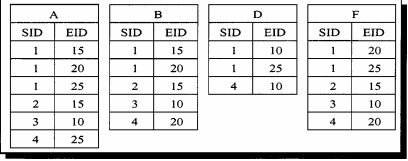
\includegraphics[width=0.5\textwidth]{figures/vertical_data.png}}
    \caption{Example of a vertical dataset}
    \label{vertical}
\end{figure}

% --------- 5. Data visualization -----------
\section{Visualization}

The visualizations were done without the use of sampling on the dataset, hence all the below plots represent all the data points in the dataset.

Each sequence in the dataset contains different websites, represented by numbers, in a particular order. To understand what the most frequently visited websites are, each event(number) in a sequence is plotted against its count in the entire dataset in Fig. \ref{website_histogram}. From this plot, it is apparent that the first website, ``frontpage'' is visited far more frequently than any of the others and is most likely to be present in the final list of frequent sequences.

\begin{figure}[h]
    \centerline{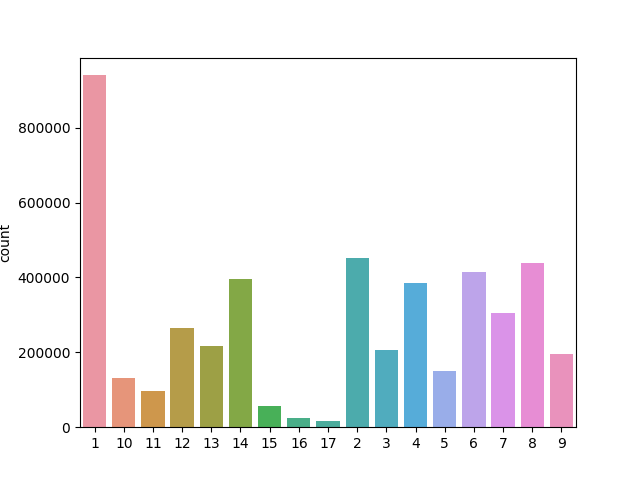
\includegraphics[width=0.5\textwidth]{figures/histogram_categories.png}}
    \caption{Plot showing number of times each website is visited}
    \label{website_histogram}
\end{figure}

The algorithm also depends on the length of each sequence and it is a good idea to know the distribution of sequence lengths in the dataset. The plot in Fig. \ref{distribution_lengths} shows the lengths of sequences in the dataset as a univariate distribution. Majority of the lengths are concentrated between 0 to 1000 with very few sequences having a length greater than 2000. The average of all the lengths in the dataset is 4.7 which can be seen from the figure with a huge portion of lengths concentrated just after 0.

\begin{figure}[h]
    \centerline{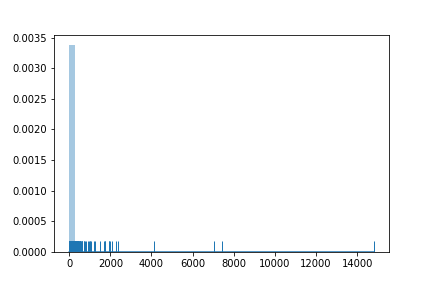
\includegraphics[width=0.5\textwidth]{figures/distribution_lengths.png}}
    \caption{Distribution of sequence lengths in the dataset}
    \label{distribution_lengths}
\end{figure}


% --------- 6. Mining tasks -----------
\section{SPADE}

\subsection{Algorithm}
The SPADE algorithm is an apriori based sequential mining technique that makes use of the vertical data format to optimize the number of scans through sequence dataset. In this data format, each element is represented as shown in Fig. \ref{vertical} and the array of sequence ID and event ID pairs is known as the ID list of that event. These ID lists carry the information necessary to find the support of the candidates(events) and also make it easy to convert to the horizontal data representation on-the-fly with less overhead. Moreover, as the length of the frequent sequence increases, the size of its ID list decreases, resulting in very fast joins.

The SPADE algorithm is roughly implemented in 3 steps:
\begin{enumerate}
    \item Find frequent items or frequent 1-sequences
    \item Find frequent 2-sequences
    \item Find frequent n-sequences recursively
\end{enumerate}

The implementation of these three steps are discussed in detail in the next section.

\subsection{Implementation}

Due to the large dataset size and also the large sequence lengths, the algorithm could not be implemented on the complete dataset. Instead, the algorithm is implemented on a subset of the data using random sampling which will approximately give the same results.

\subsubsection{Computing frequent 1-sequences}

The frequent 1-sequences are proposed to be calculated using a single scan through the vertical data format. The counts of all the unique sequences that each event occurs in are stored in a hash map and compared against the min\_sup(minimum support). This is the proposed implementation given by the SPADE paper \cite{b1} but in this project code, the frequent items are found using basic pandas operations - groupby function is used to get the id list of each event and then finding the support of unique sequence ids in each id list. If the support was greater than the min\_sup, then the event, along with it's id list, was stored as a frequent item and rest of the data was discarded.

\subsubsection{Computing frequent 2-sequences}

A naive implementation of finding the frequent 2-sequences by doing an id list join of frequent 1-sequences is very inefficient due to the number of joins needed. To counter this, the original paper proposes two methods - use a preprocessing step to gather the counts of all 2-sequences above a user specified lower bound, or  Perform a vertical-to-horizontal transformation on-the-fly and computing frequent 2-sequences from the recovered horizontal database is straight-forward. In this project, the second proposed method of converting to horizontal format on-the-fly is used. The frequent 2-sequences are then eliminated by comparing the support of each frequent sequence with the min\_sup.

\subsubsection{Computing frequent n-sequences recursively}

The final step involves recursively computing frequent sequences of all lengths greater than 2 until no more frequent sequences can be found. Frequent sequences of size n are generated by joining the id lists of two n-1 length sequences. The generation of frequent sequences is seen as a graph search problem using either BFS or DFS. During the search, although the algorithm supports pruning, the paper claims that pruning did not improve the running time and also required considerable overhead and storage to prune effectively. For these reasons, pruning was not implemented in this project.

At each step, a \textit{temporal join} is performed on two n-1 length sequences to output a sequence of length n. A temporal join between two sequences can normally lead to 3 type of outputs. But since the in the given dataset, each event consists of only a single element, a temporal join between two sequences can only have one outcome.
The implementation of the temporal join was sped up multifold by using pandas techniques and tricks. The naive implementation given by other public libraries took nearly 5 hours for the this third step but the pandas implementation took only 2 minutes on the same sample of the dataset, leading to nearly 150x speedup from the traditional implementation.

After the temporal join of each n-1 length sequence with each other, the support of all the newly generated sequences is evaluated and the sequence is added to the list of frequent sequences if it's support is greater than min\_sup. The function is then recursively called using the newly generated frequent n-sequences until no more frequent sequences are generated.


Once all the three steps are complete, frequent sequences of all lengths are obtained by combining the results of all three steps.

% --------- 7. Conclusion -----------
\section{Results}

Even though the SPADE algorithm was run only a 20\% sample of the data. The results generated are constant when tried across multiple random shuffles of the dataset. The results are shown in Table \ref{results}. These results were generated with a min\_sup of 0.05. These frequent patterns contain 13 frequent 1-sequences, 8 frequent 2-sequences, and 2 frequent 3-sequences. No joins are possible on the frequent 3 sequences hence no more sequences can be formed.

\begin{table}[htbp]
    \caption{Frequent patterns generated by SPADE}
    \label{results}
    \begin{center}
        \begin{tabular}{|c|L|}
            \hline
            \textbf{Frequent patterns} & 1, 2, 3, 4, 6, 7, 8, 9, 10, 11, 12, 13 ,14, (1,1), (1,2), (2,2), (7,7), (6,6), (4,4), (8,8), (14,14), (1,1,2), (1,2,1) \\
            \hline
        \end{tabular}
    \end{center}
\end{table}

Different combinations of min\_sup and sampling percentage were tried out on the dataset. The results in Table \ref{results} shows the generated frequent sequences for a min\_sup of 0.05 on a 20\% sample of the dataset.

\section{Conclusion}

The SPADE algorithm was implemented successfully on the given MSNBC's anonymous web dataset. This implementation is faster and more efficient than other implementations in python available online. Although the algorithm could not be run on the entire dataset at once due to hardware constraints, the algorithm gives generates the correct results on all segments of the dataset.

The only drawback of the implementation is that this code will only work on this specific type of sequential dataset, i.e, a sequential dataset with all sequences having only one element per event.

% --------- References -------s
\begin{thebibliography}{00}
    \bibitem{b1} M. Zaki, Machine Learning, vol. 42, no. 12, pp. 31-60, 2001. Available: 10.1023/a:1007652502315 [Accessed 6 July 2020].
    \bibitem{b2} Dua, D. and Graff, C. (2019). UCI Machine Learning Repository [http://archive.ics.uci.edu/ml]. Irvine, CA: University of California, School of Information and Computer Science.
\end{thebibliography}

\end{document}
